\chapter{Hiện thực và kiểm thử hệ thống}
\label{chp:05}


Chương này trình bày chi tiết quá trình hiện thực hóa kiến trúc phần cứng đã đề xuất ở các chương trước thành hệ thống vật lý trên nền tảng FPGA. Nội dung bao gồm việc tinh chỉnh lõi vi xử lý RISC-V, thiết kế cầu nối giao tiếp, tổng hợp bộ gia tốc phần cứng cho mạng nơ-ron, lập trình phần mềm nhúng điều khiển và quy trình huấn luyện, lượng tử hóa mô hình trí tuệ nhân tạo.

\section{Tổng quan hướng hiện thực}
Hệ thống gia tốc AI tại biên (Edge-AI) trong đồ án này được thiết kế theo phương pháp đồng thiết kế phần cứng/phần mềm (Hardware-Software Co-design) mang tính dị cấu trúc (Heterogeneous). Để đảm bảo tính linh hoạt (linh hoạt thay đổi mô hình AI mà không cần tổng hợp lại phần cứng) và hiệu năng cao, hệ thống được hiện thực hóa theo mô hình phân tầng kiến trúc (Layered Architecture) gồm 4 tầng (Layer) phối hợp chặt chẽ với nhau:

\begin{itemize}
    \item \textbf{Layer 1 -- Data Plane (RTL):} Bộ tăng tốc \texttt{conv\_cnn} hiện thực bằng SystemVerilog, thực thi tích chập $3 \times 3$ INT8 + requantize TFLite.
    \item \textbf{Layer 2 -- Orchestrator (Bare-metal C):} Firmware chạy trên lõi RISC-V CV32E40P, đọc bảng layer (\texttt{LAYERS[]}) và lập lịch DMA cho từng layer theo cơ chế ping-pong DDR.
    \item \textbf{Layer 3 -- Application (PYNQ Python):} Notebook Jupyter chạy trên ARM Cortex-A53 với Ubuntu PYNQ, đảm nhiệm tiền xử lý ảnh, kích hoạt RISC-V và hậu xử lý kết quả (Global Average Pool + softmax + argmax).
    \item \textbf{Layer 4 -- Toolchain (Python notebook):} Pipeline huấn luyện chạy trên Host PC (hoặc Google Colab), sinh \texttt{layer\_table.h} (cấu hình per-layer) và \texttt{weights.bin} (trọng số INT8) từ mô hình Keras đã được lượng tử hóa.
\end{itemize}

% \begin{figure}[!h]
%     \centering
%     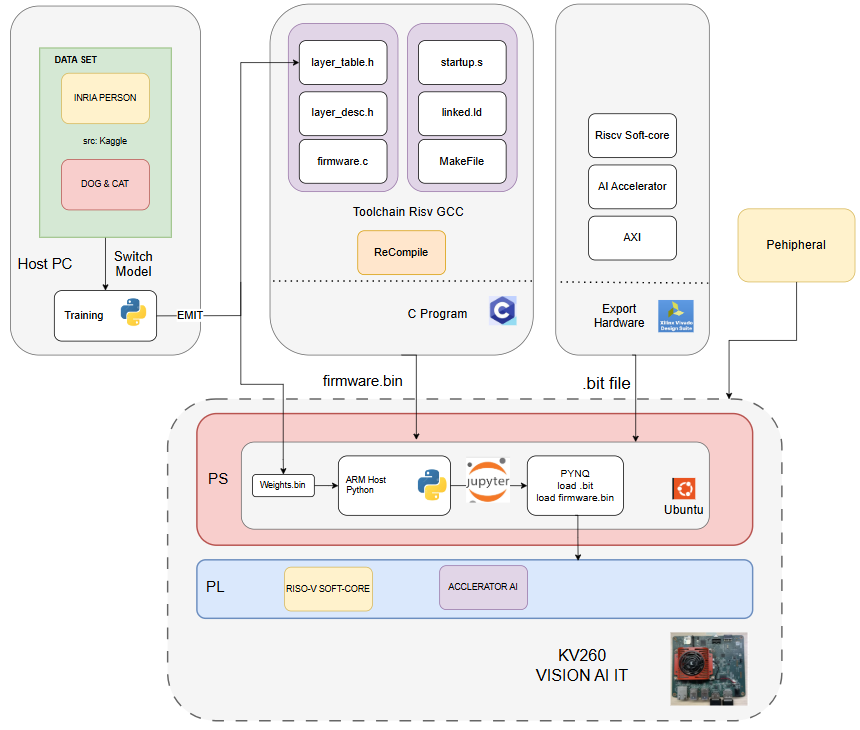
\includegraphics[width=1\linewidth]{chapter05/img/flowwork.png}
%     \caption{Sơ đồ tổng quan luồng dữ liệu giữa 4 tầng kiến trúc.}
%     \label{fig:flowwork}
% \end{figure}
% TODO: thêm hình flowwork.png khi vẽ xong block diagram 4-layer

\textbf{Quy ước giao tiếp giữa các tầng}
% Bảng artifacts (5 files)
\begin{table}[!h]
    \centering
    \caption{Các artifact trao đổi giữa các tầng trong pipeline.}
    \label{tab:artifacts}
    \begin{tabular}{|l|l|l|}
        \hline
        \textbf{Artifact} & \textbf{Sinh bởi} & \textbf{Tiêu thụ bởi} \\
        \hline
        \texttt{firmware.bin}    & RISC-V toolchain      & ARM (load vào I-BRAM)         \\
        \texttt{weights.bin}     & \texttt{train.ipynb}  & ARM (load vào DDR)            \\
        \texttt{meta.json}       & \texttt{train.ipynb}  & ARM (input quantization)      \\
        \texttt{layer\_table.h}  & \texttt{train.ipynb}  & RISC-V firmware (compile-in)  \\
        \texttt{bitstream.bit}   & Vivado synth+impl     & PYNQ Overlay                  \\
        \hline
    \end{tabular}
\end{table}

\newpage
\section{Huấn luyện và lượng tử hóa mô hình AI}
\label{sec:training_impl}

Pipeline huấn luyện được hiện thực dưới dạng một Jupyter notebook duy nhất \texttt{training/train.ipynb}, có khả năng chạy đồng thời trên Google Colab (sử dụng GPU miễn phí) và máy tính cá nhân (VSCode + Jupyter kernel). Notebook tự động phát hiện môi trường (Colab vs. local) ở cell đầu tiên và clone mã nguồn từ GitHub nếu chạy trên Colab.

\subsection{Cấu trúc pipeline 8 giai đoạn}
Notebook được tổ chức thành 8 phần (sections) tuần tự, người dùng chỉ cần chỉnh tham số ở phần ``Hyperparameters'' rồi nhấn ``Run All'' để nhận đầy đủ artifact xuất ra:

\begin{enumerate}
    \item \textbf{Environment} -- detect Colab/local, cài đặt thư viện (\texttt{tensorflow}, \texttt{kagglehub}).
    \item \textbf{Config} -- đặt \texttt{MODEL}, \texttt{DATASET}, \texttt{EPOCHS}, \texttt{BATCH\_SIZE}.
    \item \textbf{Dataset} -- tải dataset qua \texttt{kagglehub}, build pipeline \texttt{tf.data} (resize, normalize, cache, prefetch).
    \item \textbf{Model} -- khởi tạo \texttt{vgg-tiny} (hoặc các model legacy như VGG16, ResNet18 cho mục đích so sánh).
    \item \textbf{Train} -- compile + fit với Adam optimizer, sparse categorical crossentropy.
    \item \textbf{PTQ} -- chuyển mô hình FP32 sang INT8 thông qua \texttt{TFLiteConverter} với 100 batch hiệu chuẩn (\texttt{representative\_dataset}) lấy từ tập validation.
    \item \textbf{Emit} -- parse mô hình \texttt{.tflite}, sinh \texttt{layer\_table.h} (mảng C struct) và \texttt{weights.bin} (binary blob) trong thư mục \texttt{training/export/}.
    \item \textbf{Distribute} -- đóng gói artifact thành ZIP để tải xuống và \texttt{rsync} lên board KV260.
\end{enumerate}

\subsection{Kiến trúc \texttt{vgg-tiny} đề xuất}
Mô hình \texttt{vgg-tiny} là một mạng \textit{fully-convolutional} gồm 5 lớp Conv $3 \times 3$ stride-1 với padding VALID, sử dụng nguyên tắc đơn giản hóa để tránh các op chưa được bộ tăng tốc Conv-CNN v2.0 hỗ trợ (như Pool, Dense, Depthwise). Bảng~\ref{tab:vgg_tiny_layers} đã trình bày chi tiết kiến trúc trong chương~\ref{chp:04}.

\begin{lstlisting}[language=Python, caption={Kiến trúc Tiny-VGG đề xuất (file \texttt{edge\_train/models.py}).}]
def build_vgg_tiny(num_classes, input_shape=(128,128,3)):
    inp = tf.keras.Input(shape=input_shape)
    x = layers.Conv2D(8,  3, activation='relu', padding='valid')(inp)
    x = layers.Conv2D(16, 3, activation='relu', padding='valid')(x)
    x = layers.Conv2D(32, 3, activation='relu', padding='valid')(x)
    x = layers.Conv2D(64, 3, activation='relu', padding='valid')(x)
    x = layers.Conv2D(num_classes, 3, activation=None, padding='valid')(x)
    x = layers.GlobalAveragePooling2D()(x)
    return tf.keras.Model(inp, layers.Softmax()(x), name='vgg-tiny')
\end{lstlisting}

\subsection{Lượng tử hóa sau huấn luyện (Post-Training Quantization)}
Quá trình PTQ áp dụng kỹ thuật \textit{Integer-Arithmetic-Only Inference} của Jacob et al. \cite{jacob2018quantization} (đã trình bày tại mục~\ref{sec:quantization_theory}). Cụ thể trong notebook:

\begin{itemize}
    \item Sau khi mô hình FP32 đạt độ chính xác mục tiêu, \texttt{tf.lite.TFLiteConverter} được khởi tạo với \texttt{optimizations = [DEFAULT]}.
    \item Tham số \texttt{representative\_dataset} được gán bằng một generator lấy 100 batch từ tập validation -- đây là bước \textit{calibration} để xác định dải $[\min, \max]$ của activations cho từng layer.
    \item Tham số \texttt{inference\_input\_type} và \texttt{inference\_output\_type} đặt là \texttt{INT8} để buộc TFLite quantize cả input/output, giúp giảm bước dequantize ở runtime.
    \item Sau khi \texttt{convert()}, file \texttt{.tflite} thu được chứa đầy đủ trọng số INT8, scale và zero-point per-tensor cho từng layer.
\end{itemize}

\subsection{Trình biên dịch tự sinh \texttt{layer\_table.h} và \texttt{weights.bin}}
\label{ssec:emitter}
Module \texttt{edge\_train/emit.py} thực hiện vai trò ``compiler'' bằng cách parse mô hình \texttt{.tflite} (sử dụng FlatBuffer schema chính thức của TensorFlow Lite) và sinh hai artifact đồng bộ:

\begin{itemize}
    \item \textbf{\texttt{layer\_table.h}} -- mảng \texttt{layer\_desc\_t LAYERS[NUM\_LAYERS]} dưới dạng C header. Mỗi entry chứa: kích thước IFM (\texttt{w\_in}, \texttt{h\_in}), số kênh (\texttt{cin}, \texttt{cout}), offset trong \texttt{weights.bin}, hệ số $M_{q31}$ và $n$, zero-point đầu ra, cờ \texttt{has\_relu}. Tổng cộng 40 byte/layer.
    \item \textbf{\texttt{weights.bin}} -- binary blob chứa toàn bộ trọng số INT8 và bias INT32 nối tiếp nhau theo thứ tự layer. ARM tải file này vào DDR và RISC-V dùng \texttt{LAYERS[i].weight\_offset} để truy cập đúng vị trí cho từng layer.
\end{itemize}

Hàm \texttt{quantize\_multiplier()} chuyển hệ số nhân float $M = (s_{\mathrm{in}} \cdot s_{\mathrm{w}})/s_{\mathrm{out}}$ sang dạng cố định Q31 + dịch phải:
\begin{equation}
    M_{q31}, n = \texttt{quantize\_multiplier}\!\left(\frac{s_{\mathrm{in}} \cdot s_{\mathrm{w}}}{s_{\mathrm{out}}}\right)
\end{equation}
Hàm sử dụng \texttt{math.frexp()} của Python để tách $M$ thành significand và exponent, từ đó có $M_{q31} = \mathrm{round}(\text{significand} \cdot 2^{31})$ và $n = -\text{exponent}$. Trường hợp $M \geq 1$ (chưa được hỗ trợ bởi RTL hiện tại) sẽ được clip về giá trị max và in cảnh báo.

\newpage
\section{Hiện thực khối gia tốc phần cứng Conv\_CNN v2.0}
\label{sec:cnn-ip}

Bộ tăng tốc \texttt{conv\_cnn} v2.0 được hiện thực hóa dưới dạng một IP core độc lập trong Vivado IP Repository (\texttt{hw/ip\_repo/conv\_cnn\_1\_0}), với 3 giao diện AXI: \texttt{S00\_AXI} (control AXI4-Lite), \texttt{S00\_AXIS} (input stream cho IFM/weights), \texttt{M00\_AXIS} (output stream cho OFM). IP được thiết kế lại hoàn toàn từ phiên bản v1.x (Sobel-only, hardcode trọng số) thành kiến trúc tổng quát hỗ trợ Conv $3 \times 3$ INT8 đầy đủ với requantize TFLite.

\subsection{Tổng quan kiến trúc Conv\_CNN v2.0}
% Datapath block diagram
\begin{figure}[!h]
    \centering
    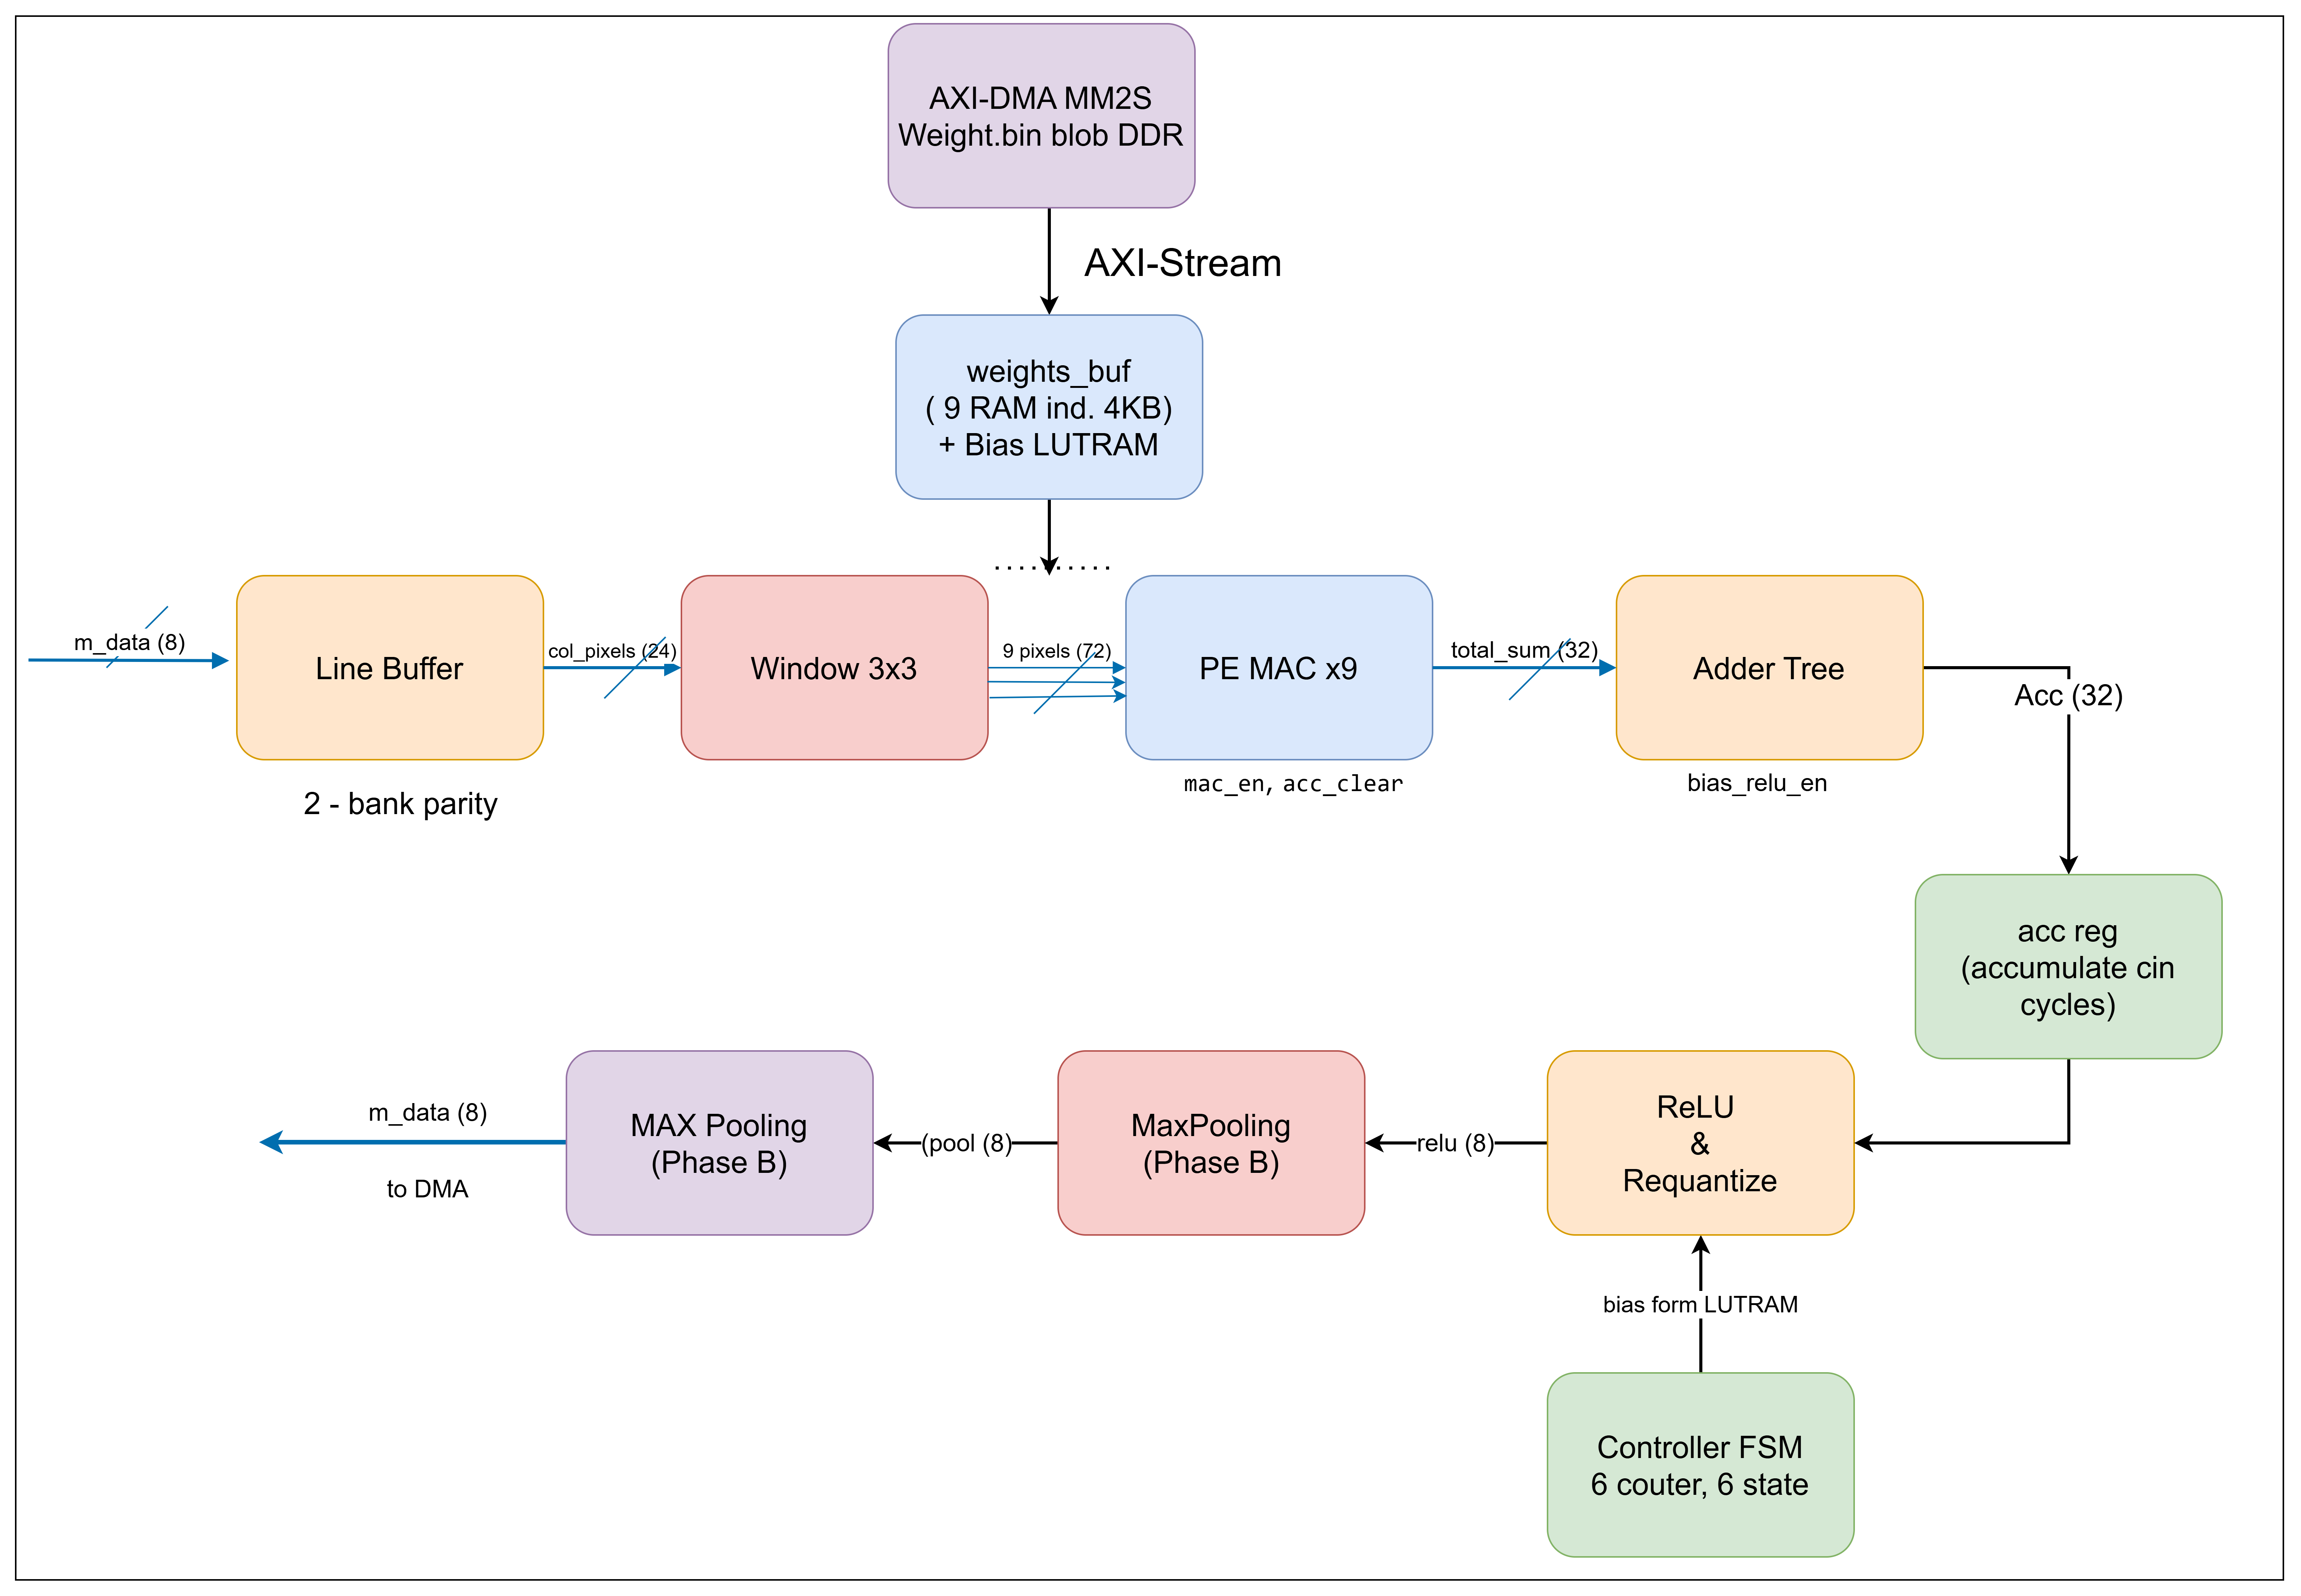
\includegraphics[width=1\textwidth]{chapter05/img/conv_cnn_datapath.png}
    \caption{Sơ đồ datapath conv\_cnn IP: từ AXIS in qua line buffer,
    window, MAC array, requantize đến AXIS out.}
    \label{fig:conv-cnn-datapath}
\end{figure}

Datapath gồm 7 module chính phối hợp qua một FSM trung tâm:
\begin{itemize}
    \item \texttt{conv\_pkg.sv} -- package tham số (giới hạn kích thước, độ rộng datatype, độ trễ pipeline).
    \item \texttt{controller\_fsm.sv} -- FSM 6 trạng thái, 6 bộ đếm điều phối luồng kênh-xen-kẽ và iteration trên \texttt{cnt\_cout}.
    \item \texttt{line\_buffer.sv} -- 2 bank BRAM cho 2 hàng pixel cũ, ping-pong theo parity hàng.
    \item \texttt{window\_3x3.sv} -- mảng thanh ghi $3 \times 3 \times \texttt{MAX\_CIN}$ giữ cửa sổ tích chập hiện tại.
    \item \texttt{weight\_buf.sv} -- 9 BRAM độc lập cho weights + LUTRAM cho bias INT32.
    \item \texttt{pe\_mac.sv} -- 9 PE MAC INT8$\times$INT8 song song (DSP48E2-mappable).
    \item \texttt{requantize.sv} -- pipeline 3-tầng: cộng bias, nhân $M_{q31}$, dịch phải, cộng zero-point, bão hòa, ReLU.
\end{itemize}

\subsection{Tham số hóa và package \texttt{conv\_pkg.sv}}
Toàn bộ tham số bound (\texttt{MAX\_WIDTH}, \texttt{MAX\_CIN}, \texttt{MAX\_COUT}) và độ rộng datatype được đặt trong \texttt{conv\_pkg.sv}, cho phép scale tài nguyên mà không sửa từng module. Phiên bản hiện tại đặt \texttt{MAX\_WIDTH = 128}, \texttt{MAX\_CIN = MAX\_COUT = 64} -- vừa đủ cho \texttt{vgg-tiny} mà không phình tài nguyên không cần thiết. Việc đẩy lên cho mạng lớn hơn (như VGG11) chỉ cần thay tham số trong package và re-synthesize.

\subsection{Khối điều khiển \texttt{controller\_fsm.sv}}
FSM gồm 6 trạng thái (\texttt{S\_IDLE}, \texttt{S\_ACCEPT\_CIN}, \texttt{S\_LATCH\_WIN}, \texttt{S\_COMPUTE}, \texttt{S\_WAIT\_REQUANT}, \texttt{S\_EMIT}) phối hợp với 6 bộ đếm để duyệt 3 vòng lặp lồng nhau:

\begin{lstlisting}[language=Verilog, caption={Trình tự duyệt 3 vòng lặp trong controller FSM}, label={lst:fsm}]
for (y_in, x_in raster scan):                  // outer
    for (cin in 0..num_cin-1): receive 1 IFM    // channel-interleaved
    if (window valid):
        for (cnt_cout in 0..num_cout-1):        // middle
            mac_clear; for (cnt_cin in 0..num_cin-1) mac_enable
            requant_in_valid -> wait latency -> emit M_AXIS
\end{lstlisting}

Cơ chế \textit{channel-interleaved per pixel} cho phép pipeline IFM input liên tục: tại mỗi vị trí pixel, FSM nhận \texttt{num\_cin} samples (một sample/cycle) trước khi cửa sổ trượt qua vị trí kế. Số chu kỳ tính toán cho mỗi pixel output xấp xỉ $\texttt{num\_cout} \times (\texttt{num\_cin} + L_{\mathrm{requant}} + 1)$.

\subsection{Bộ đệm dòng và cửa sổ \texttt{line\_buffer.sv}, \texttt{window\_3x3.sv}}
Để thực hiện tích chập $3 \times 3$, tại mỗi thời điểm cần 3 hàng pixel liên tiếp cùng lúc. Module \texttt{line\_buffer.sv} sử dụng \textbf{2 bank BRAM} mỗi bank dung lượng $\texttt{MAX\_W} \times \texttt{MAX\_CIN}$ byte với cơ chế \textit{read-before-write parity-toggled}: khi pixel mới ghi vào bank này thì hai hàng cũ vẫn được giữ ở bank kia, tránh ghi đè dữ liệu đang đọc. Độ trễ đọc BRAM 1 chu kỳ được FSM bù trừ bằng pipeline alignment register.

Module \texttt{window\_3x3.sv} là một mảng thanh ghi $3 \times 3 \times \texttt{MAX\_CIN}$, dịch cột mỗi khi tín hiệu \texttt{shift\_cols} được nhả. Khi cần đọc 9 pixel cho một kênh \texttt{cnt\_cin} cụ thể, mảng cung cấp đầu ra tổ hợp ngay trong chu kỳ đó (không có thanh ghi đầu ra), giảm độ trễ tính toán.

\subsection{Bộ nhớ trọng số \texttt{weight\_buf.sv} -- bài học về BRAM inference}
\label{ssec:weight_buf_bram}
Một trong những vấn đề nan giải trong quá trình hiện thực hóa là Vivado synth không suy luận đúng BRAM cho mảng trọng số. Phiên bản đầu tiên sử dụng mảng 3D unpacked \texttt{[K\_TAPS][MAX\_COUT][MAX\_CIN]} với reset đồng bộ, dẫn đến tổng hợp ra \textbf{295,000 FFs} (FDRE -- thanh ghi flip-flop) thay vì BRAM, vượt xa tài nguyên FPGA cho phép.

Sau khi tách thành \textbf{9 mảng 2D độc lập} (mỗi mảng tương ứng 1 trong 9 vị trí kernel) và bỏ lệnh reset đồng bộ, Vivado mới suy luận đúng thành \textbf{9 RAMB18 / 4 KB mỗi block}, tổng 36 KB. Bias INT32 lưu trong LUTRAM (do số lượng nhỏ -- tối đa 64 entry). Đây là một trong những bài học kỹ thuật quan trọng được rút ra: cấu trúc dữ liệu trong RTL có ảnh hưởng quyết định đến việc Vivado suy luận BRAM hay FF -- và sự khác biệt về tài nguyên có thể lên đến vài bậc độ lớn.

Cơ chế nạp weights theo từng layer được điều khiển bởi cờ \texttt{mode\_load} trong thanh ghi \texttt{CTRL}: khi \texttt{mode\_load = 1}, FSM chuyển sang trạng thái nhận stream từ \texttt{S00\_AXIS} và ghi tuần tự vào 9 BRAM + LUTRAM bias. Khi nạp xong, RISC-V đặt \texttt{mode\_load = 0} và bắt đầu chế độ infer.

\subsection{Mảng MAC và cây cộng \texttt{pe\_mac.sv}}
Mỗi PE thực hiện $a_{\mathrm{int8}} \times w_{\mathrm{int8}} \to \mathrm{int32}$ rồi cộng vào thanh ghi tích lũy 32-bit. Cấu trúc với 2 thanh ghi pipeline (MREG sau nhân, PREG sau cộng) cho phép Vivado ánh xạ trực tiếp vào DSP48E2 với 1 DSP/PE. 9 PE chạy song song xử lý đồng thời 9 vị trí của kernel $3 \times 3$, đầu ra được tổng hợp qua \textit{adder tree} 4-tầng (combinational) để cho ra một giá trị tích chập 32-bit/cycle.

Đối với mạng có \texttt{cin > 1}, kết quả của 9 PE được tích lũy thêm qua \texttt{cin} chu kỳ trong thanh ghi \texttt{acc[31:0]} trước khi xuất sang khối requantize. Tổng cộng cần $9 \times \texttt{cin}$ phép nhân INT8 cho mỗi điểm OFM.

\subsection{Khối lượng tử hóa lại \texttt{requantize.sv}}
\label{ssec:requantize}
Khối requantize hiện thực công thức TFLite \cite{jacob2018quantization}:
\begin{equation}
    y_{q} = \mathrm{sat}_{\mathrm{INT8}}\!\left(
        \left\lfloor \frac{(\sum_{i,j,c} x \cdot w + b) \cdot M_{q31} + 2^{30+n}}{2^{31+n}} \right\rfloor + z_{\mathrm{out}}
    \right)
\end{equation}

Pipeline 3-tầng:
\begin{itemize}
    \item \textbf{Tầng 1 -- bias add:} cộng bias INT32 (đọc từ LUTRAM) với accumulator 32-bit.
    \item \textbf{Tầng 2 -- multiply $M_{q31}$:} nhân INT32 $\times$ INT31 thành INT63, có làm tròn round-half-up (cộng $2^{30+n}$ trước khi dịch).
    \item \textbf{Tầng 3 -- shift + zero-point + saturate + ReLU:} dịch phải $31 + n$ bit qua barrel shifter, cộng zero-point INT8, bão hòa về dải $[-128, 127]$, kẹp về $[0, 127]$ nếu \texttt{has\_relu = 1}.
\end{itemize}

\subsection{Tích hợp tổng thể qua AXI}
% S00_AXI register map (Bảng 5.x)
% AXI-Stream IFM/OFM
\begin{table}[htbp]
    \centering
    \caption{Bản đồ thanh ghi điều khiển S00\_AXI (32 bytes, 8 thanh ghi).}
    \label{tab:s00-axi-regs}
    \begin{tabular}{|c|l|c|l|}
        \hline
        \textbf{Offset} & \textbf{Tên} & \textbf{R/W} & \textbf{Layout} \\
        \hline
        0x00 & GEOMETRY  & RW & width[15:0], height[31:16] \\
        0x04 & CTRL      & RW & start, pool\_en, mode\_load, has\_relu \\
        0x08 & STATUS    & RO & done \\
        0x0C & CHANNELS  & RW & num\_cin[15:0], num\_cout[31:16] \\
        0x10 & M\_Q31    & RW & Q31 multiplier \\
        0x14 & SHIFT\_ZP & RW & shift[5:0], output\_zp[15:8] \\
        \hline
    \end{tabular}
\end{table}

Trình tự lập trình một layer (do firmware RISC-V thực hiện trong \texttt{process\_one\_layer()}):
\begin{enumerate}
    \item Ghi \texttt{GEOMETRY}, \texttt{CHANNELS}, \texttt{M\_Q31}, \texttt{SHIFT\_ZP} cho layer hiện tại.
    \item Ghi \texttt{CTRL.mode\_load = 1, CTRL.start = 1} (load mode), DMA stream weights tới \texttt{S00\_AXIS}, poll \texttt{STATUS.done}.
    \item Đặt \texttt{CTRL.has\_relu, CTRL.start = 1} (infer mode), DMA stream IFM tới \texttt{S00\_AXIS}, OFM được M00\_AXIS đẩy về DDR qua S2MM.
    \item Poll \texttt{STATUS.done = 1}, hạ \texttt{CTRL.start = 0}, chuyển sang layer tiếp theo.
\end{enumerate}

\subsection{Đánh giá khối tăng tốc CONV-CNN}

\begin{figure}[!h]
    \centering
    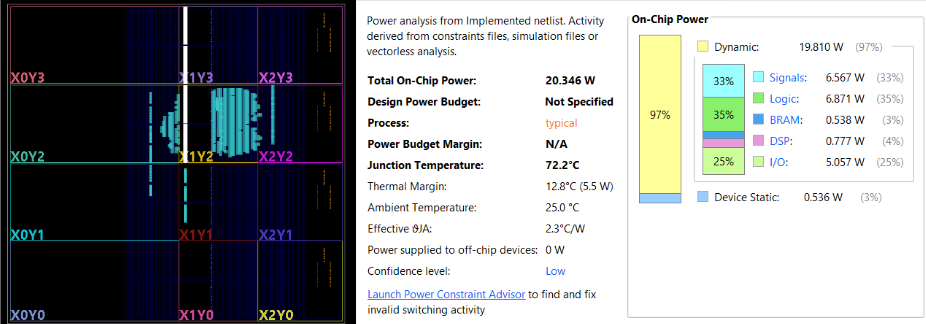
\includegraphics[width=1\linewidth]{chapter05/img/cnn_imple.png}
    \caption{Báo cáo chạy khối CNN}
    \label{fig:overall}
\end{figure}

\begin{figure}[!h]
    \centering
    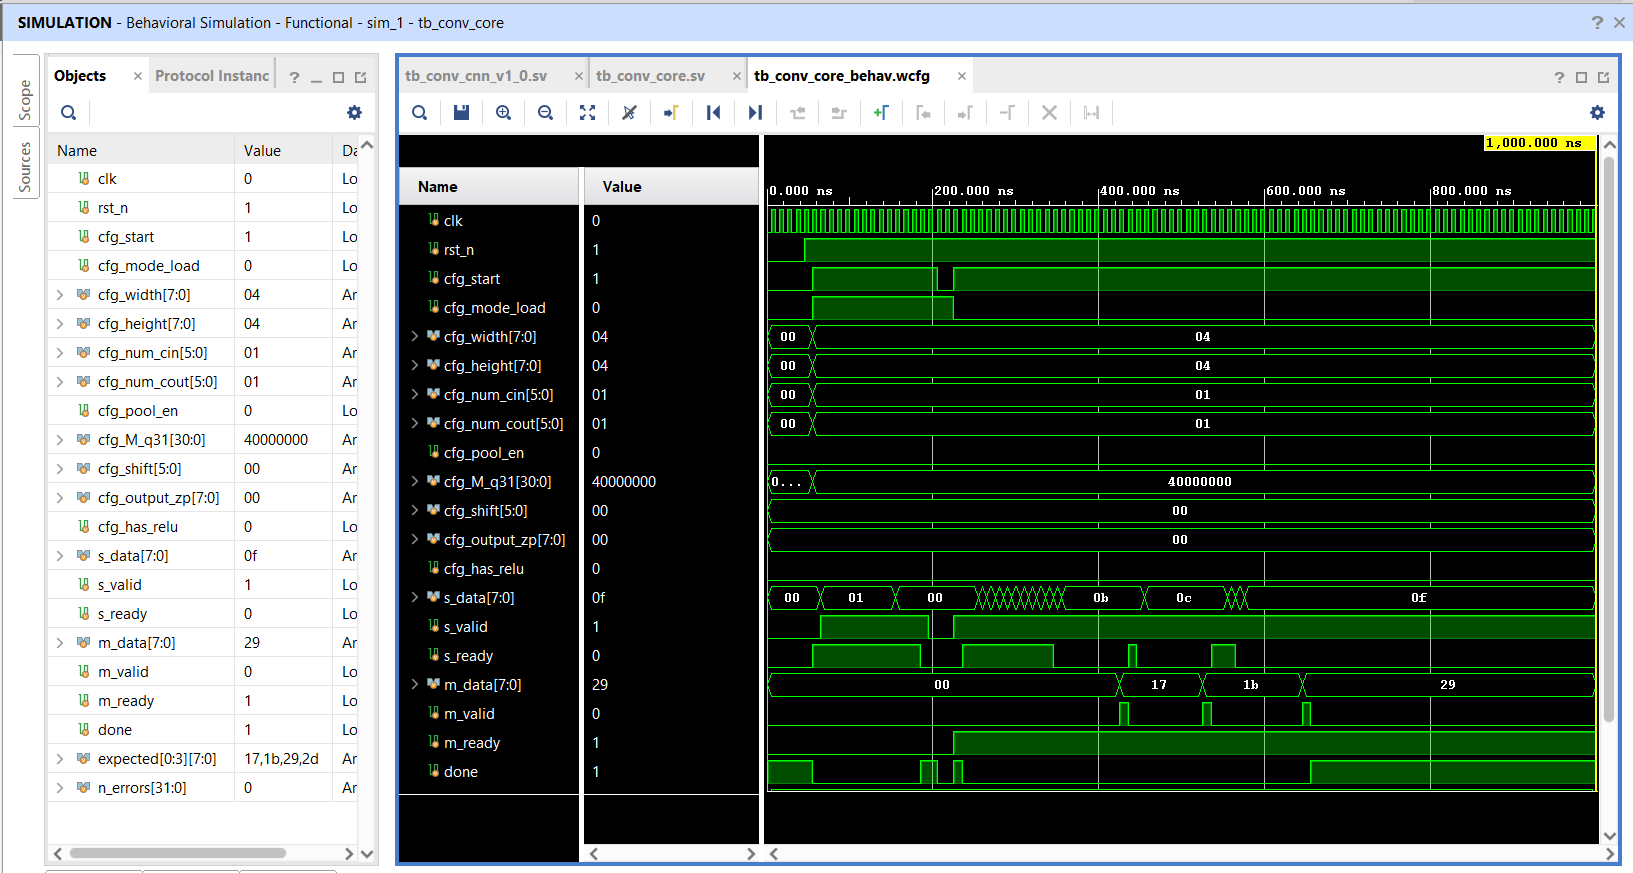
\includegraphics[width=1\linewidth]{chapter05/img/cnn_waveform.png}
    \caption{Kết quả chạy simulate khối CNN}
    \label{fig:waveform}
\end{figure}

\newpage
\section{Hiện thực RISC-V Soft-core}
\subsection{Tinh chỉnh CV32E40P Core}
Lõi vi xử lý CV32E40P mã nguồn mở nguyên bản được thiết kế với đầy đủ các tập lệnh mở rộng, bao gồm cả khối xử lý số thực dấu phẩy động (FPU - Floating Point Unit). Tuy nhiên, để tối ưu hóa tài nguyên phần cứng (LUT, FF, DSP) trên chip FPGA cho bộ tăng tốc trí tuệ nhân tạo, lõi CPU đã được tinh chỉnh lại ở mức mã nguồn RTL.

Cụ thể, toàn bộ khối xử lý số thực và các lệnh liên quan (tập lệnh mở rộng F) đã được loại bỏ. Sự tinh giản này là hoàn toàn hợp lý do toàn bộ mô hình học sâu trong hệ thống đã được lượng tử hóa xuống kiểu dữ liệu số nguyên 8-bit (INT8). Vi xử lý lúc này chỉ hoạt động với tập lệnh cơ bản RV32IMC, chịu trách nhiệm điều phối luồng điều khiển, quản lý ngắt và cấu hình thanh ghi thay vì tham gia tính toán trực tiếp. Bên cạnh đó, bộ giải mã lệnh (Instruction Decoder) cũng được tùy biến để tối ưu hóa đường truyền dữ liệu, loại bỏ các khối logic không cần thiết, giúp cải thiện tần số hoạt động tối đa (Fmax) của lõi.

\subsection{Hiện thực cầu nối giao tiếp OBI sang AXI4 (OBI to AXI)}
\label{sec:obi_axi}
Giao thức giao tiếp bộ nhớ mặc định của lõi CV32E40P là OBI (Open Bus Interface). Tuy nhiên, nền tảng thiết kế SoC của Xilinx Vivado sử dụng chuẩn giao tiếp AMBA AXI4 làm nòng cốt. Để tích hợp thành công lõi RISC-V vào bản vẽ hệ thống cùng với khối xử lý trung tâm (PS) và các bộ nhớ đệm, một cầu nối giao tiếp (Bridge) chuyển đổi từ tín hiệu OBI sang AXI4 đã được thiết kế và hiện thực.

Cầu nối này (\texttt{obi\_to\_axi.sv}) bao gồm hai luồng độc lập: một luồng dành cho việc nạp lệnh (Instruction Fetch) và một luồng dành cho truy xuất dữ liệu (Data Access). Khối logic bên trong sử dụng \texttt{fifo\_v3} để theo dõi các giao dịch outstanding (\texttt{MaxRequests = 4}), thực hiện nhiệm vụ biên dịch các tín hiệu điều khiển OBI (\textit{req}, \textit{gnt}, \textit{rvalid}) thành các kênh AXI4-Lite tương ứng (AR, R, AW, W, B). Quá trình kiểm thử mô phỏng (\texttt{tb\_riscv\_top.sv}) xác nhận cầu nối không gây ra trạng thái tắc nghẽn (Deadlock) và xử lý chính xác cả các tín hiệu báo lỗi đường truyền.

\subsection{Đóng gói IP \texttt{riscv\_top}}
Toàn bộ wrapper \texttt{riscv\_top.sv} (gồm CV32E40P + 2 instance \texttt{obi\_to\_axi}) được đóng gói thành Vivado IP \texttt{hw/ip\_repo/riscv\_top\_1\_0} với 3 cổng external bổ sung:
\begin{itemize}
    \item \texttt{fetch\_enable\_i} -- ARM điều khiển boot/halt qua AXI GPIO.
    \item \texttt{irq\_conv\_cnn\_i} -- ngắt level từ \texttt{conv\_cnn.irq} được map vào MFAST0 (\texttt{mip[16]}).
    \item \texttt{core\_sleep\_o} -- trạng thái WFI để ARM poll.
\end{itemize}

\newpage
\section{Hiện thực Firmware RISC-V (Layer 2 -- Orchestrator)}
\label{sec:firmware}

Firmware RISC-V được viết bằng ngôn ngữ C bare-metal (không có hệ điều hành), biên dịch bằng \texttt{riscv-none-elf-gcc} với cờ \texttt{-march=rv32imc -mabi=ilp32}. Toàn bộ \texttt{.text + .rodata} (bao gồm \texttt{LAYERS[]} từ \texttt{layer\_table.h}) được nạp vào I-BRAM 64 KB, còn \texttt{.data + .bss + stack} nằm ở D-BRAM 256 KB.

\subsection{Tổ chức bộ nhớ -- linker script}
File \texttt{linked.ld} định nghĩa hai vùng nhớ split:

\begin{lstlisting}[language=C, caption={Trích đoạn linker script \texttt{firmware/linked.ld}.}]
MEMORY {
    IRAM (rx)  : ORIGIN = 0x00000000, LENGTH = 64K  /* I-BRAM: .text, .rodata */
    DRAM (rwx) : ORIGIN = 0xB0040000, LENGTH = 256K /* D-BRAM: .data, .bss, stack */
}
\end{lstlisting}

Stack được khởi tạo tại \texttt{ORIGIN(DRAM) + LENGTH(DRAM) = 0xB008\_0000} bởi \texttt{startup.s} -- file assembly chứa reset handler: thiết lập \texttt{sp}, zero-out \texttt{.bss}, sao chép \texttt{.data} từ ROM (nếu có) và nhảy đến \texttt{main()}.

\subsection{Vòng đời driver \texttt{main.c}}
Hàm \texttt{main()} chạy theo polling loop đơn giản (chế độ ngắt được dành cho phiên bản tối ưu sau):

\begin{lstlisting}[language=C, caption={Polling loop chính của firmware.}]
int main(void) {
    while (1) {
        if (mmio_r32(REG_CMD_FROM_ARM) == CMD_START) {
            mmio_w32(REG_STATUS_TO_ARM, STATUS_BUSY);
            uint32_t base_w = mmio_r32(REG_WEIGHT_BASE);
            uint32_t buf_a  = mmio_r32(REG_IFM_PHYS_ADDR);
            uint32_t buf_b  = mmio_r32(REG_OFM_PHYS_ADDR);
            for (int i = 0; i < NUM_LAYERS; i++) {
                uint32_t in  = (i & 1) ? buf_b : buf_a;
                uint32_t out = (i & 1) ? buf_a : buf_b;
                process_one_layer(&LAYERS[i], base_w, in, out);
            }
            mmio_w32(REG_STATUS_TO_ARM, STATUS_DONE);
            mmio_w32(REG_CMD_FROM_ARM, CMD_IDLE);
        }
    }
}
\end{lstlisting}

Hàm \texttt{process\_one\_layer()} thực hiện đầy đủ trình tự 4 bước (mục~\ref{sec:cnn-ip}): nạp weights qua DMA, lập trình DMA cho IFM/OFM, kích hoạt conv\_cnn ở chế độ infer, và poll \texttt{STATUS.done}. Ping-pong DDR giữa \texttt{buf\_a} và \texttt{buf\_b} đảm bảo OFM của layer $i$ được làm IFM cho layer $i+1$ mà không cần phân bổ buffer riêng.

\newpage
\section{Hiện thực Host Runtime (Layer 3 -- PYNQ Application)}
\label{sec:host_runtime}

Tầng ứng dụng chạy trên ARM Cortex-A53 dưới Ubuntu PYNQ Image (Kria-PYNQ v3.0), sử dụng thư viện PYNQ để tải bitstream, cấp phát buffer DDR cache-coherent (CMA) và viết MMIO. Mã nguồn được tổ chức thành package \texttt{host/edge\_ai/} (4 module ngắn) phục vụ cả notebook lẫn CLI.

\subsection{Cấu trúc package \texttt{host/edge\_ai/}}
\begin{itemize}
    \item \texttt{constants.py} -- bản đồ thanh ghi (\texttt{REG\_*}), cờ trạng thái (\texttt{STATUS\_*}, \texttt{CMD\_*}), tên IP BRAM. \textbf{Phải đồng bộ với \texttt{firmware/main.c}}.
    \item \texttt{overlay.py} -- class \texttt{EdgeAIOverlay} bọc \texttt{pynq.Overlay}, cung cấp các method \texttt{load\_firmware()}, \texttt{kick()}, \texttt{poll\_done(timeout)}, \texttt{set\_io\_buffers(buf\_a, buf\_b)}.
    \item \texttt{preprocess.py} -- \texttt{cv2.imread} $\to$ resize $128 \times 128$ $\to$ INT8 quantize (đọc \texttt{input\_scale}, \texttt{input\_zero\_point} từ \texttt{meta.json}).
    \item \texttt{postprocess.py} -- Global Average Pool trên trục $(H, W)$ + dequantize float + softmax + argmax.
\end{itemize}

\subsection{Quy trình tải bitstream và boot RISC-V}
\begin{lstlisting}[language=Python, caption={Trình tự khởi động hệ thống trong notebook (rút gọn).}]
from edge_ai.overlay import EdgeAIOverlay
ov = EdgeAIOverlay("kria_soc_wrapper.bit")  # auto-loads .hwh

# Reset RISC-V, nap firmware vao I-BRAM, release reset
ov.load_firmware("firmware.bin")             # axi_bram_ctrl_2 Port B
ov.release_riscv_reset()                     # axi_gpio fetch_enable_i = 1

# Cap phat 3 buffer DDR cache-coherent (CMA)
import pynq, numpy as np
wbuf  = pynq.allocate(shape=(WEIGHTS_SIZE,),  dtype=np.int8)
buf_a = pynq.allocate(shape=(MAX_OFM_BYTES,), dtype=np.int8)
buf_b = pynq.allocate(shape=(MAX_OFM_BYTES,), dtype=np.int8)

# Nap weights.bin va publish dia chi vat ly cho RISC-V
wbuf[:] = np.fromfile("vgg-tiny_cats_dogs.weights.bin", dtype=np.int8)
wbuf.flush()
ov.set_weights_addr(wbuf.physical_address)
ov.set_io_buffers(buf_a.physical_address, buf_b.physical_address)
\end{lstlisting}

\subsection{Inference loop trong notebook}
Sau khi setup xong, phần lặp thực thi cho mỗi ảnh (cell ``2.3 DMA + kick + poll'' trong \texttt{inference\_demo.ipynb}):

\begin{enumerate}
    \item \texttt{img\_q = preprocess\_image(path, meta)} -- đọc + resize + quantize INT8.
    \item \texttt{buf\_a[:] = img\_q.flatten(); buf\_a.flush()} -- ghi IFM vào CMA buffer.
    \item \texttt{ov.kick()} -- ghi \texttt{CMD\_START} qua MMIO, RISC-V phát hiện và bắt đầu duyệt LAYERS[].
    \item \texttt{ov.poll\_done(timeout=2.0)} -- chờ \texttt{STATUS\_TO\_ARM == STATUS\_DONE}.
    \item Đọc OFM cuối từ \texttt{buf\_a} hoặc \texttt{buf\_b} (xác định bởi \texttt{meta['fpga']['final\_ofm\_buf\_idx']}), gọi \texttt{.invalidate()} trước khi đọc.
    \item \texttt{cls, conf = postprocess.gap\_argmax(ofm, scale, zp)} -- GAP $\to$ softmax $\to$ argmax.
\end{enumerate}

Notebook \texttt{benchmark.ipynb} bổ sung sweep accuracy + latency trên toàn tập validation, vẽ confusion matrix và histogram độ trễ để đánh giá hiệu năng end-to-end.

\newpage
\section{Tích hợp Block Design trong Vivado}

\label{sec:bd}
\begin{figure}[H] % cần \usepackage{float}
\centering

\includegraphics[width=\linewidth]{chapter05/img/arch.png}
\caption{Sơ khối minh họa hệ thống}
\label{fig:arch}
\end{figure}


\begin{figure}[H]
\centering
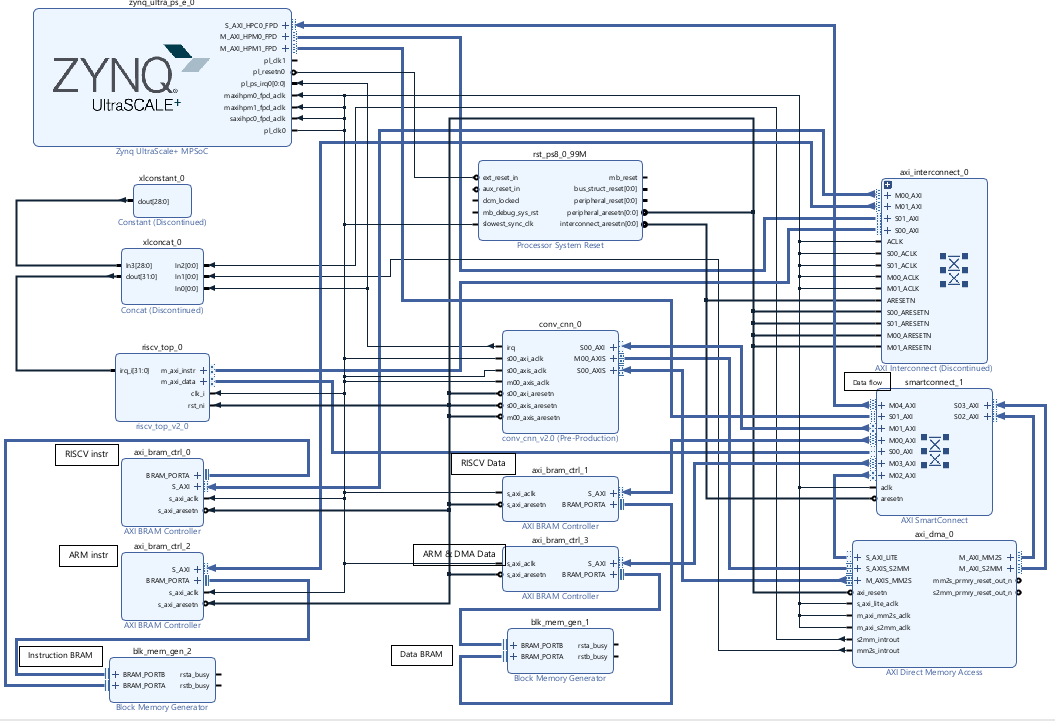
\includegraphics[width=1.2\linewidth, angle=90]{chapter05/img/arch_vivado.png}
\caption{Thiết kế khối trong vivado}
\label{fig:arch_vivado}
\end{figure}


\newpage
\subsection{Bản đồ bộ nhớ và Address Editor}
% RISC-V view, ARM view, DMA view
% BD validation issues đã giải quyết
\begin{figure}[h]
    \centering
    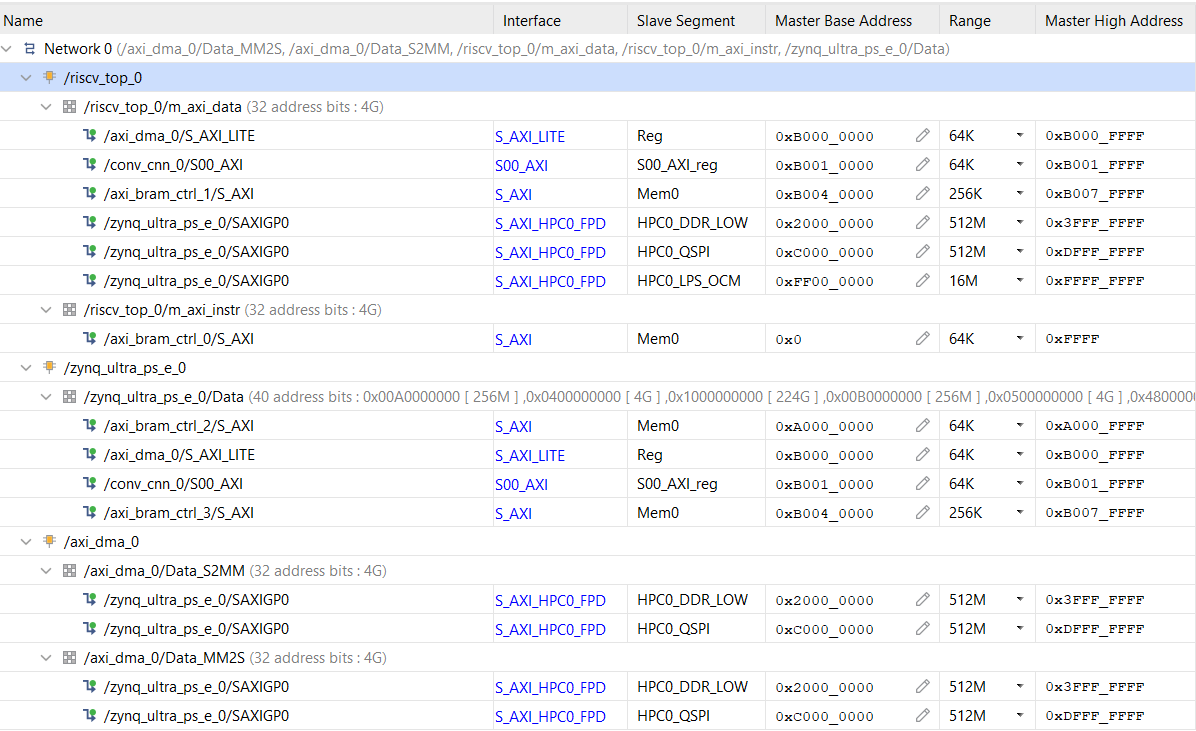
\includegraphics[width=1\linewidth]{chapter05//img/address_editor.png}
    \caption{Bảng chia section trong bộ nhớ}
    \label{fig:address_editor}
\end{figure}

Quá trình tích hợp Block Design ban đầu phát sinh 6 cảnh báo từ Vivado Address Editor (2 errors BD~41-1267 + 4 critical warnings) do SmartConnect mặc định mở route từ \texttt{axi\_dma\_0/Data\_MM2S/S2MM} đến \texttt{axi\_bram\_ctrl\_1} (D-BRAM Port A của RISC-V). Vấn đề được giải quyết bằng 3 thao tác trong Address Editor:

\begin{enumerate}
    \item Đồng bộ offset RISC-V $\leftrightarrow$ PS để cùng slave có cùng địa chỉ logic (cùng nằm trong dải \texttt{0xB0xx\_xxxx}).
    \item Exclude DMA $\to$ BRAM (DMA chỉ thấy DDR qua \texttt{S\_AXI\_HPC0\_FPD}, không thấy BRAM).
    \item Exclude RISC-V $\to$ \texttt{axi\_bram\_ctrl\_3} (RISC-V chỉ ghi Port A của D-BRAM, Port B dành riêng cho ARM).
\end{enumerate}

Sau khi fix, validate sạch (0 errors / 0 critical warnings), bitstream được tổng hợp thành công.

\newpage
\subsection{Đồng bộ ARM \(\leftrightarrow\) RISC-V qua D-BRAM dual-port}
% Bảng register layout shared region
Mặc dù D-BRAM 256~KB là một khối BRAM duy nhất ở mức vật lý, nó được cấu hình dual-port (RAMB36 trên Ultrascale+) với hai \texttt{axi\_bram\_ctrl} riêng biệt (Port A cho RISC-V, Port B cho ARM). Phần đầu của vùng nhớ này được dành cho các thanh ghi handshake (Bảng~\ref{tab:handshake-regs-ch5}), giúp ARM và RISC-V trao đổi command/status với độ trễ cực thấp (zero round-trip qua DDR).

\begin{table}[h]
    \centering
    \caption{Bố cục thanh ghi handshake D-BRAM Port B (offset từ \texttt{0xB004\_0000}).}
    \label{tab:handshake-regs-ch5}
    \begin{tabular}{|l|l|l|p{4.5cm}|}
        \hline
        \textbf{Offset} & \textbf{Tên} & \textbf{Hướng} & \textbf{Mô tả} \\ \hline
        +0x00 & \texttt{CMD\_FROM\_ARM}    & ARM $\to$ RISC-V & \texttt{0x01} = START \\ \hline
        +0x04 & \texttt{STATUS\_TO\_ARM}   & RISC-V $\to$ ARM & IDLE / BUSY / DONE \\ \hline
        +0x08 & \texttt{DATASET\_ID}       & ARM $\to$ RISC-V & 0 = INRIA, 1 = cats\_dogs \\ \hline
        +0x18 & \texttt{IFM\_PHYS\_ADDR}   & ARM $\to$ RISC-V & DDR addr buffer A \\ \hline
        +0x1C & \texttt{OFM\_PHYS\_ADDR}   & ARM $\to$ RISC-V & DDR addr buffer B \\ \hline
        +0x20 & \texttt{WEIGHT\_BASE}      & ARM $\to$ RISC-V & DDR addr weights blob \\ \hline
    \end{tabular}
\end{table}

\newpage
\section{Quy trình kiểm thử}
\label{sec:testing}

Hệ thống được kiểm thử theo phương pháp tiếp cận \textit{nhiều tầng} (multi-level testing) để cô lập lỗi sớm: từ unit testbench RTL $\to$ tích hợp IP $\to$ đối chiếu golden vector $\to$ kiểm thử end-to-end trên board.

\subsection{Kiểm thử đơn vị (Unit Testbench)}
% TB từng module: requantize, FSM, line_buffer
% Vector test thủ công
Mỗi module RTL chính có testbench riêng kiểm tra hành vi cô lập với input có chủ đích:
\begin{itemize}
    \item \texttt{tb\_requantize} -- vector hoá trị đầu vào dải $[-2^{20}, 2^{20}]$, đối chiếu với reference Python (Q31 mul + barrel shift) để xác nhận round-half-up đúng.
    \item \texttt{tb\_line\_buffer} -- ghi tuần tự một frame $128 \times 128$, kiểm tra parity-toggle giữ nguyên 2 hàng cũ khi hàng mới được ghi.
    \item \texttt{tb\_riscv\_top.sv} -- behavioral instr memory đáp NOP, kiểm tra fetch advance qua \texttt{m\_axi\_instr}.
\end{itemize}

\subsection{Kiểm thử tích hợp IP}
\label{ssec:tb-ip}
Testbench \texttt{tb\_conv\_core.sv} mô phỏng toàn bộ luồng load + infer
với input 4×4×1, weights toàn 1, M=0.5, kỳ vọng OFM = $\{23, 27, 41, 45\}$
(với round-half-up).

\begin{equation}
    y_{q} = \mathrm{sat}_{\mathrm{INT8}}\!\left(
        \left\lfloor \frac{(\sum_{i,j,c} x \cdot w + b) \cdot M_{q31} + 2^{30+n}}{2^{31+n}} \right\rfloor + z_{\mathrm{out}}
    \right)
\end{equation}

\subsection{Đối chiếu với golden vector từ TFLite Interpreter}
% Bit-exact comparison strategy
% Per-tensor vs per-axis quant note
Để đảm bảo tính đúng đắn của RTL trước khi kiểm thử trên board, mỗi layer của \texttt{vgg-tiny} được chạy song song bằng \texttt{tf.lite.Interpreter} (đã quantize INT8) trên Host PC. Đầu ra OFM của TFLite được lưu thành mảng INT8 và so sánh \textbf{bit-exact} với OFM mà testbench RTL sinh ra. Cách so sánh này hiệu quả vì TFLite cũng dùng đúng công thức Q31 multiplier với round-half-up, do đó không có sai số làm tròn giữa hai phía.

Một lưu ý kỹ thuật quan trọng: TFLite mặc định dùng \textit{per-axis quantization} cho weight (mỗi cout-channel có scale riêng), trong khi RTL hiện tại chỉ hỗ trợ \textit{per-tensor} (1 scale cho cả layer). Do đó pipeline emit phải force convert sang per-tensor (\texttt{disable\_per\_channel = True}) -- điều này gây giảm độ chính xác khoảng 0.5--2\% trên các layer sâu, là một đánh đổi đã được cân nhắc kỹ trong giai đoạn thiết kế.

\subsection{Kiểm thử trên board KV260}
% Hardware-in-the-loop methodology
% Dataset split (train/val/test)
Sau khi qua đủ các tầng kiểm thử mô phỏng, hệ thống được triển khai xuống board Kria KV260 thật:

\begin{itemize}
    \item \textbf{Triển khai:} Script \texttt{deploy.sh} sử dụng \texttt{rsync} để đồng bộ 4 nhánh artifact (\texttt{hw/artifacts/} -- bitstream + .hwh; \texttt{firmware/firmware.bin}; \texttt{training/export/} -- weights + meta.json; \texttt{host/} -- Python package + notebooks) từ PC sang board qua SSH.
    \item \textbf{Sanity check:} Chạy \texttt{inference\_demo.ipynb} với một ảnh test đơn lẻ, kiểm tra latency, và visual hóa kết quả classification.
    \item \textbf{Đánh giá hệ thống:} Chạy \texttt{benchmark.ipynb} qua toàn bộ tập validation, ghi nhận \textit{accuracy} và \textit{latency} cho mỗi ảnh.
    \item \textbf{Hardware-in-the-loop comparison:} Mỗi ảnh được chạy đồng thời qua (i) TFLite Interpreter trên ARM (reference), và (ii) Conv-CNN trên FPGA. Đầu ra logits được so sánh; sai khác nếu có thường < 1 LSB do thứ tự cộng dồn floating ở pipeline ARM.
\end{itemize}

Kết quả định lượng (accuracy, latency, sai số) được trình bày chi tiết tại chương~\ref{chp:06}.
